\subsection{Decoding the MDS Magic: What Does It Mean for Receivers?}

\begin{tcolorbox}[colback=gray!10, colframe=black, title=E4C07] What does the MDS of a receiver represent? 
\begin{enumerate}[label=\Alph*.]
    \item The meter display sensitivity
    \item \textbf{The minimum discernible signal}
    \item The modulation distortion specification
    \item The maximum detectable spectrum
\end{enumerate} \end{tcolorbox}

\subsubsection{Understanding MDS}

MDS stands for Minimum Discernible Signal. It is a measure that represents the smallest signal level that a receiver can reliably detect above the noise floor. In practical terms, it signifies the receiver's sensitivity to incoming signals. The lower the MDS value, the weaker the signal the receiver can detect, which is crucial for applications such as weak signal communications.

\subsubsection{Related Concepts}

To understand MDS fully, we must explore a few key concepts in radio communication:

\begin{itemize}
    \item \textbf{Signal-to-Noise Ratio (SNR):} This is a measure of the level of the desired signal to the level of background noise. A higher SNR indicates better quality of the signal received.
    
    \item \textbf{Noise Figure (NF):} This parameter quantifies how much noise a receiver adds to the signal it receives. It is essential to consider NF when evaluating the overall performance of a receiver.
    
    \item \textbf{Receiver Sensitivity:} This is often expressed in terms of MDS. It indicates how well a receiver can operate under poor signal conditions.
\end{itemize}

Additionally, the MDS is often expressed in dBm (decibels relative to one milliwatt). For example, if a receiver has an MDS of -100 dBm, it means it can detect signals that are as weak as 1 picowatt with confidence, making this information vital for planning communication systems that rely on detecting faint signals.

\subsubsection{Calculation Example}

To illustrate how MDS can be calculated, consider the following equation:

\[
\text{MDS (dBm)} = \text{Noise Floor (dBm)} + \text{SNR threshold (dB)}
\]

For a receiver with a noise floor of -110 dBm and a required SNR of 10 dB for proper signal discernment, we compute:

\[
\text{MDS} = -110 \text{ dBm} + 10 \text{ dB} = -100 \text{ dBm}
\]

Thus, this receiver would have an MDS of -100 dBm. 

\subsubsection{Diagram Representation}

Below is a simple diagram expressing the noise floor and the MDS:

\begin{center}
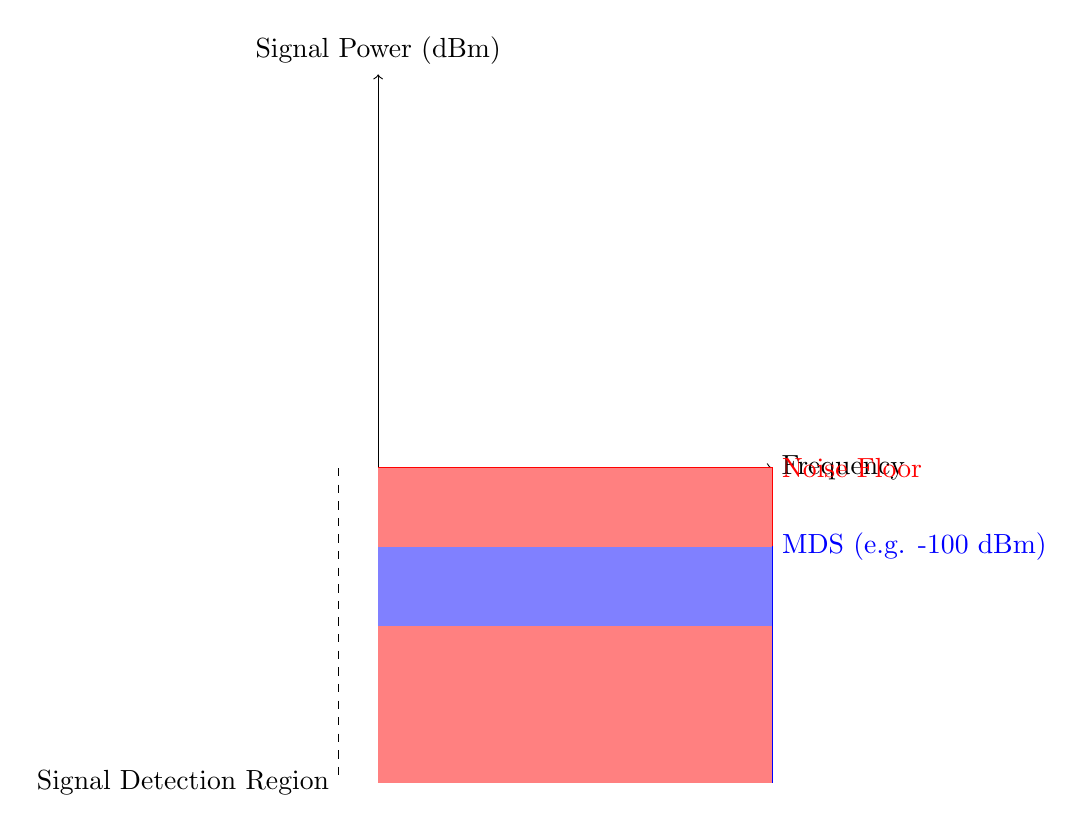
\begin{tikzpicture}
    \draw[->] (0,0) -- (0,5) node[above] {Signal Power (dBm)};
    \draw[->] (0,0) -- (5,0) node[right] {Frequency};
    
    \draw[thick, red] (0,0) -- (5,0) node[right] {Noise Floor} -- (5,-3);
    \draw[thick, blue] (0,-1) -- (5,-1) node[right] {MDS (e.g. -100 dBm)} -- (5,-4);
    
    \draw[dashed] (-0.5,0) -- (-0.5,-4) node[left] {Signal Detection Region};
    
    \fill[red!50] (0,-4) rectangle (5,0);
    \fill[blue!50] (0,-2) rectangle (5,-1);
\end{tikzpicture}
\end{center}
